\documentclass{article}
\usepackage{graphicx}
\let\bs\textbackslash
\def\pc{\bigskip\obeylines\parindent=0pt}
\def\tisbl{\noindent\parindent=0pt\obeylines\catcode`\|=0 \catcode`\#=12\catcode`\%=12 \catcode`\\=12 \catcode`\_=12 \tt}
\def\tb{\bigskip\tisbl}
\begin{document}
{\noindent\bf\LARGE TISBL language specification}

\noindent Rob Mitchelmore

\subsubsection*{Revision history}
\begin{description}
\item[2.0] First \LaTeX version.  Massive expansion of the original, and rethink of some syntax.
\item[1.0] The original HTML version from 2004.
\end{description}

\section{Language overview}

\subsection{Introduction}

TISBL is an extremely simple and very definitely unusable stack-based language influenced by FORTH, PostScript, LISP, \TeX, and which punctuation characters looked pretty.

TISBL has no code blocks and no real idea of scope; nor are there any named functions or variables; it also has a somewhat blurred distinction between code and data.

Abandon hope, all ye who enter here.

\subsection{Making the computer ignore you}

Comments are introduced with a \texttt{\%} sign and continue to the end of the line:

{\tb % everything from here to EOL is ignored}

\subsection{Simple operations}

TISBL is a stack machine; each TISBL subprogram (more on this later; for the moment, you can assume that each program is a subprogram) has two data stacks and an execution stack.
There are two basic data types in TISBL: word and number. A word is an arbitrary string of characters (although for syntactic reasons, a literal word cannot have whitespace within it); a number is either an integer or a floating-point number.

To push a word onto the stack, prefix it with a \texttt{'} (single quote). For example:

{\tb 'hello % pushes the word "hello" onto the stack} 

\bigskip\noindent To push an number, use the \# character; for example:

{\tb #3 % pushes the number 3 onto the stack}

\bigskip \noindent Multiple tokens can be seperated with any amount of whitespace (being either the space character, tabs, or carriage returns and/or linefeeds). For example:

{\tb
#3 #4

|bigskip #3
#4

|bigskip|textrm{and} #3 |quad|quad #4
}

\bigskip\noindent are all equivalent, pushing 3, then 4 onto the stack.

To perform operations upon the stack, verbs are invoked. A verb consists of a backslash (\bs ) followed by one or more characters that are not whitespace and not full stop (.), comma (,), colon (:) or semicolon (;). A verb pulls its input from the stack and pushes its results back to the stack. For example:

{\tb #3 #4 \+}

\bigskip\noindent pushes 3 and 4 onto the stack, adds them (\bs + attempts to pop two arguments from the stack), and pushes 3+4 onto the stack. To output, use \bs out:

{\tb #3 #4 \+ \out}

\bigskip\noindent produces '7' on the screen, as expected.

The verbs available by default are listed in the standard library section of this document, below.

\subsection{Using the second data stack}

Each TISBL execution context has two data stacks; the primary one which has been used so far, and a second one, which is called '\texttt{:}' for no particularly good reason.

To push data onto a stack other than the main one, place the stack's name before the type marker, for example:

{\tb :#3}

\bigskip\noindent pushes 3 onto the second data stack. To invoke a verb, the verb must be given two stacks: one from which to read the input, which goes after the backslash but before the name, and one onto which to post the output, which goes after the name, for example:

{\tb \dup:}

\bigskip\noindent which copies an item from the top of the main data stack to the second data stack,

{\tb \:dup}

\bigskip\noindent which copies an item from the top of the second data stack to the main data stack,

{\tb \:swap:}

\bigskip\noindent which swaps the top two items of the secondary stack, and

{\tb :#3 :#4 \:+}

\bigskip\noindent which adds 3 and 4 from the secondary data stack and pushes the result onto the main data stack.

\subsection{Novel uses of \bs rm: or, the execution stack}

When a TISBL program is loaded, what is actually loaded from the text file is the initial state of the execution stack, each token being put onto the stack as a word, with the first token in the file as the head of the stack (this is to ensure some semblance of normal execution order). To execute the program, each word is popped off the execution stack and executed; thus the top of the execution stack is always the next token to be executed. Once loaded, and once the program is running, the execution stack becomes another stack accessible to the program; its name is '\texttt{,}'. For example:

{\tb \,rm}

\bigskip\noindent which skips the next token (removes the head of the execution stack),

{\tb \,dup,}

\bigskip\noindent which will make the next token execute twice, and on a more convoluted note:

{\tb :'#3 :'4 \:+: \:dup,}

\bigskip\noindent which produces a word ``\#34" on the second data stack and copies that to the execution stack; the end result of this being to push 34 onto the main data stack. A more confusing, and rather crueller, variant on this would be:

{\tb :':# :#34 \:+ \dup,}

\bigskip\noindent this constructs a ``:\#34" word on the main data stack from the ``:\#" word and the 34 number on the second data stack, then copies that ``:\#34" from the main data stack onto the execution stack, thus causing the number 34 to be pushed to the second data stack as the next operation.

Phew.

\subsection{Code blocks, \bs exec and \bs verb}

\bigskip\noindent Consider for a moment the following code:

{\tb ''hello ''world '\+ '\out}

\bigskip\noindent After this, the primary data stack will consist of:

{\tb TOP => '\out, '\+, ''world, ''hello}

\bigskip\noindent If one then executes

{\tb #4 \multipop:}

\bigskip\noindent the second data stack will look like:

{\tb TOP => ''hello, ''world, '\+, '\out}

\bigskip\noindent Note that the order of the tokens has been effectively reversed in the transfer between stacks, as \bs multipop moves items one at a time. If instead of pushing onto the second data stack, however, one pushes onto the execution stack, then the tokens will be executed and "helloworld" will be output.

The \bs exec verb extends this concept by creating a new subprogram and doing a multipop onto its execution stack.  A subprogram has its own primary and secondary data stacks, and things written to these stacks will not affect the world outside the subprogram.  For example:

{\tb ''aaa '#3 '#4 '\+ '\out
#5 \exec}

\bigskip\noindent will print, as expected, 7; and when the subprogram ends, the remaining item (\texttt{'aaa}) on its main data stack is discarded:

{\tb ''aaa '#3 '#4 '\+ '\out
#5 \exec \out}

\bigskip\noindent will give a stack underflow error when it hits the \bs out.

There is also a facility in TISBL to add verbs to the language, and this is done with the \bs verb verb. \bs verb first pops a word from the stack, and then a code block as \bs exec does, and associates the word with the code block in the global 'verb pool'. When the verb is executed, the code block is executed in a new subprogram as if it was \bs exec-ed. For example:

{\tb '#3 '#4 '\+ '\out #4
'seven \verb}

\bigskip\noindent defines a verb that outputs "7" called "seven"; and calling this verb:

{\tb \seven}

\bigskip\noindent will execute that subprogram and output "7".

\subsection{Talkative Subprograms}

So far, the subprograms examined have had a major shortcoming:  they cannot take parameters and push back results. This shortcoming is addressed by the fact that each subprogram has a reference to an input stack and an ouput stack, much as the built-in verbs have. A subprogram cannot write to its input stack, and cannot read from its output stack; these stacks are both referred to as '.', and the correct stack is used depending on context. For example:

{\tb .'hello}

\bigskip\noindent pushes the word "hello" onto the current subprogram's output stack, while

{\tb \.+}

\bigskip\noindent pops the two arguments for + from the current subprogram's input stack and pushes the result onto the primary data stack; and

{\tb \.dup.}

\bigskip\noindent which duplicates the top of the input stack onto the top of the output stack.

When the subprogram is executed, the input and output stacks of the block are filled in from the verb that caused the execution; in the case of \bs exec, the input and output stacks passed to \bs exec, and in the case of \bs verbed code blocks, the input and output stacks passed to the verb name. For example:

{\tb #3.5
'\.mv '#2 '\* '\dup. #4 \exec:}

\bigskip\noindent puts \#7.0 onto the second data stack (the code and the input were from the main stack as passed as the input stack to \bs exec; the output goes to ':' as that is the output stack to \bs exec). Another example:

{\tb '\.mv '#2 '\* '\dup. #4 'timestwo \verb
#3.5 \timestwo:}

\bigskip\noindent is equivalent to the \bs exec example above. More interesting things can be done with verbs, however:

{\tb '\.timestwo '\timestwo. #2 'timesfour \verb}

\bigskip\noindent which defines a timesfour verb in term of timestwo, using the '.' notation for input and output stacks.

\subsection{\bs if and \bs while}

\bs if implements conditionals, and works as follows: First, it pops a code block from its input stack as \bs exec does; then it pops a single item from its input stack. If that item is not 0 then it executes the block as a subprogram as if it had been run with \bs exec, inheriting its input and output stacks from the \bs if verb. Otherwise, the code block is discarded. An example:

{\tb 'this \_
#1 '.'will #1 \if
#0 '.'won't #1 \if
\+ \_ 'be \_ \+ 'executed. \+ \out}

\bigskip\noindent which will always produce "this will be executed."; as the \#0 in the second \bs if will prevent that code block from being executed.

The \bs while construct is a variant on this. It too first pops a code block from its input stack, then it pops an item and if it isn't 0, executes the code block. While \bs if stops there, however, \bs while continues: when the code block has finished executing, it pops another item, and if it isn't 0, executes the code block again in a new subprogram (data stacks are not persistent between iterations in a \bs while - it works much like repeated calls to \bs exec on an identical code block); and it continues thus until it pops a 0, whereupon it stops and allows the program to continue. An example is:

{\tb #0 #1 #2 #3 #4
'\.dup '\out #2 \while}

\bigskip\noindent which produces the output

{\tb 3210}

\bigskip\noindent The \#4 is never printed, as the \bs while swallows the first item remaining on the stack each iteration. By making the input and output stacks of \bs while the same, it is possible to implement something akin to the while loop in other languages, by pushing something back onto the output stack at the end of the loop:

{\tb #100 #1
'\.mv '#1 '\- '\dup. '\dup. '\out #6 \while}

\bigskip\noindent which produces the numbers from 100 to 0. 

This example is slightly more convoluted than previous ones; so, a dissection. The 100 is the number to count down from; the \#1 is the initial loop condition. This item must be present as \bs while takes one item before evaluating the code block for the first time. Thus, when the code block executes for the first time, there is only the 100 left on the stack. The code block then moves that 100 to its own local stack, subtracts 1 from it, duplicates it twice back onto the parent stack (remember, \bs while will swallow one item, and one needs to remain on the parent stack as the datum for the next iteration). It then outputs the number and ends. The \bs while then pops the top of its stack, finds that it is not 0, and iterates again.

\subsection{Messing With the Future, Part 2}

In TISBL, subprograms have the ability to mess with their parent context's execution stack (thus removing its single sole possible remaining purpose, that of a fairly secure programming language). The parent's execution stack is called ';', in a move designed to annoy Java, C, and Pascal programmers who are used to putting a semicolon at the end of each (or most) lines, as this way there will be no syntax error, but the program is likely to do something violently unpredictable.

Note that while the subprogram is running, its parent is frozen; thus, any instructions pushed onto ; will not be executed until the subprogram has finished executing. For example:

{\tb ''hello '\_ '\out ';'\world #4 'hello \verb
''world '\n '\out #3 'world \verb
\hello}

\bigskip\noindent would output

{\tb hello world}

\bigskip\noindent as the ``hello" verb forces the program to execute ``\bs world" following it by pushing the ``\bs world'' word onto its caller's execution stack. Another, even more useless example:

{\tb ''hello '\_ '\out ';'\hello #4 'hello \verb \hello}

\bigskip\noindent which outputs "hello hello hello hello ..." until the user gets bored and kills the interpreter\footnote{On interpreters which buffer their output, like the THINK Pascal one, you may see no output at all.}.

\subsection{A note on syntax checking}

It is important to note that a TISBL interpreter should not check each token for correct formatting as it is loaded, but only as it is executed; for example:

{\tb 'hello \_ \out /error 'world}

\bigskip\noindent should not bail out until execution of the token "/error" is attempted.




\section{Language spec}

This outlines an interpreter for TISBL.  Algorithms are illustrative only and should be viewed with appropriate levels of critical thinking.  Equivalent or entertainingly non-equivalent implementations are still conforming for what little that is worth.

\subsection{Interpreter state}

The interpreter state consists of a stack of \emph{contexts}.  When the program starts the state contains one context.

Each context consists of three stacks:

\begin{itemize}
\item A primary stack.
\item A secondary stack.
\item An execution stack.
\end{itemize}

\noindent It also consists of three references to other stacks:

\begin{itemize}
\item Its input stack
\item Its output stack
\item Its parent's execution stack
\end{itemize}

\noindent Implementations may limit the depth of the context stack.
The interpreter state also contains a single, global verb table.  Each entry in this table consists of a verb name and the initial execution stack for a context.

\subsection{Stacks}

A stack must provide three primitive operations:

\begin{description}
\item[Push] which pushes an item onto the stack
\item[Pop] which removes the top item from the stack and returns it.
\item[Peek] which returns the top item from the stack without removing it.
\end{description}

Each item in the stack may be:

\begin{itemize}
\item A string
\item An integer
\item A floating-point number
\end{itemize}

Integers should be at least 16 bits wide.  What kind of float is used is implementation-specific.  Strings may be either Unicode, Latin-1 or ASCII.  If implementations really want to use EBCDIC I suppose they may.

\subsection{Running a context}

To run a context:

\begin{itemize}
\item While the execution stack is not empty:
\begin{itemize}
\item Pop an item from the execution stack
\item Parse it
\item Execute the parsed representation
\end{itemize}
\end{itemize}

\subsection{Parsing a token}

A token consists of

\begin{itemize}
\item What kind of token it is: number, word or verb.
\item The name of its input stack, if it is a verb.
\item The name of its output stack
\item Its contents.
\end{itemize}

\noindent In order to parse a token:

\begin{itemize}
\item Is the first character a backslash ({\tt \textbackslash})?
\item If so:
\begin{itemize}
\item Chop the backslash off
\item Attempt to read a stack character (see below).
\item If you get one, store a reference to the stack it represents in the token's input stack field and chop the character off.
\item If you don't, store a reference to the default data stack in the token's input stack field.
\item Look at the last character; if it is a valid stack character, then read it and store a reference to the stack it represents in the token's output stack field.  Chop off the stack character.
\item What remains is the contents of the token.
\end{itemize}

\item Otherwise: (the first character is not a backslash)
\begin{itemize}
\item Attempt to read a stack character (see below)
\item If you get one, store a reference to the stack it represents in the token's output stack field and chop the character off.
\item Attempt to read a hash (\#) or a single quote (').  If you get the former, store that the token is a number.  If the latter, store that it is a word.  If you get neither, bail out.
\item The remainder of the string is the contents of the token.
\end{itemize}
\end{itemize}

\noindent A stack character is one of a full stop (.), a colon (:), a comma (,) or a semicolon (;).

\subsection{Executing a token}

To execute a token:

\begin{itemize}
\item If the token is a word, then push the contents of the token onto the token's specified output stack as a string item.
\item If the token is a number then:
\begin{itemize}
\item If the contents of the token contains a decimal point (.), convert the contents into an implementation-dependent float format and push that onto the token's specified output stack.
\item Otherwise, convert the contents of the token into an integer and push that onto the token's specified input stack.
\item Should the content of the token not convert to being a number, bail out.
\end{itemize}
\item If the token is a verb, then:
\begin{itemize}
\item If the content of the verb matches the name of a verb in the verb table (\emph{case-sensitive!}) then
\begin{itemize}
\item Start a new context
\item Set the contents of the execution stack of the new verb to be that matching the verb name in the verb table (\emph{preserving ordering})
\item Set the input and output stacks of the context according to the input and output stacks of the token.
\item Execute the new context (see above)
\item Clean up context as necessary.
\end{itemize}
\item Otherwise, if the content of the verb matches the name of a standard library function, run it
\item Otherwise, bail out.
\end{itemize}
\end{itemize}

\subsection{Loading a file}

A file consists of a set of whitespace-separated tokens.  Comments begin with a percent sign (\%) either at the beginning of a line or after a whitespace and continue until the end of the line.  A state machine for this is:

\begin{center}
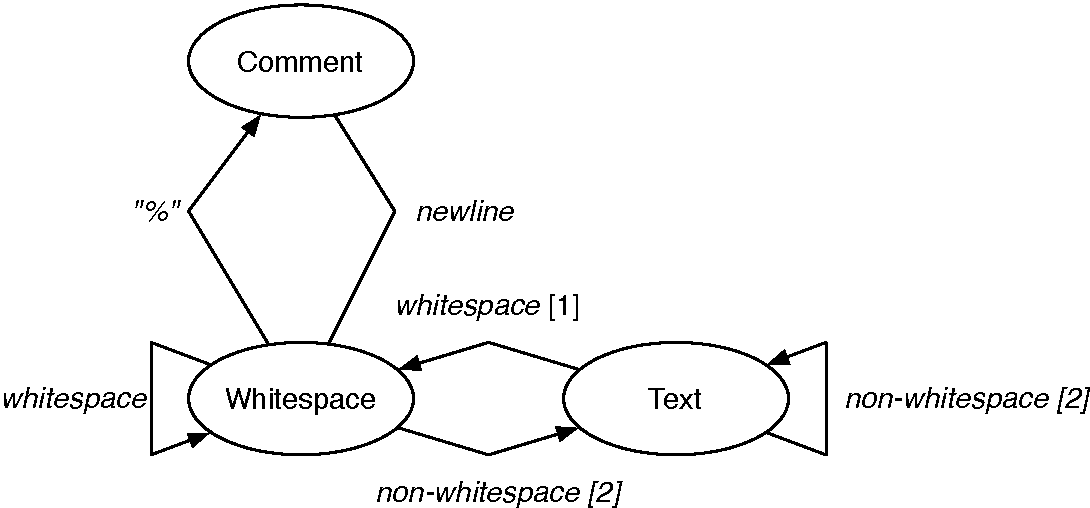
\includegraphics[width=0.7\columnwidth]{tisbl-sm}
\end{center}

\subsubsection*{Notes [referring to the bits in square brackets]}

\begin{enumerate}
\item If the buffer that you're using to assemble the token is not empty, put its contents onto the \emph{bottom} of the initial execution stack then clear the buffer.
\item Append the character to the buffer
\end{enumerate}

\noindent To load a file:

\begin{itemize}
\item Create an initial context with invalid input and output stacks.
\item Parse the input file according to the above state machine.
\item Execute the initial context.
\end{itemize}

\section{Standard Library}
\subsection{\bs trace=0 and \bs trace=1}

Should set a bit of internal state for debug; when trace=1 the interpreter should print the contents of the primary, secondary and execution stacks before every token is executed.

\subsection{\bs exec}

\bs exec creates a new context with the same input and output stacks as itself; it pops an integer from its input stack, then pops that number of elements from its input stack, pushing each one onto the execution stack of the new context.
{\pc
$exec(input, output) \rightarrow$
\quad $ctx \leftarrow$ new Context
\quad $ctx.input \leftarrow input$
\quad $ctx.output \leftarrow output$
\quad $count \leftarrow pop(input)$
\quad die unless $count$ is a integer
\quad for $i$ in $[1..count]$ do
\quad \quad $item \leftarrow pop(input)$
\quad \quad $push(ctx.exec, item)$
\quad execute $ctx$
}

\subsection{\bs verb}

\bs verb creates a new verb in the verb table.  First, it creates a new stack.  It pops a string from its input stack to be the name of the verb and stores it, then pops an integer from its input stack.  It pops this number of elements from its input stack, pushing them onto the new stack as it goes.  It then adds a mapping from the name to the new stack to the verb table.

{\pc
$verb(input,output) \rightarrow$
\quad $s \leftarrow$ new Stack
\quad $name \leftarrow pop(input)$
\quad die unless $name$ is a string
\quad $count \leftarrow pop(input)$
\quad die unless $count$ is an integer
\quad for $i$ in $[1..count]$ do
\quad \quad $item \leftarrow pop(input)$
\quad \quad $push(s, item)$
\quad add $(name, s)$ to verb table
}

\subsection{\bs if}

\bs if conditionally executes code.  First, it creates a new context with the input and output stacks set the same as those on the verb.  Then, it pops an integer from its input stack, and pops that number of elements from its input stack, pushing each onto the execution stack of the new context as it goes.  It then pops an element from its input stack; if that element is a number and 0, then it discards the new context.  Otherwise, it executes it.

{\pc
$if(input,output) \rightarrow$
\quad $ctx \leftarrow$ new Context
\quad $ctx.input \leftarrow input$
\quad $ctx.output \leftarrow output$
\quad $count \leftarrow pop(input)$
\quad die if $count$ is not an integer
\quad for $i$ in $[1..count]$ do
\quad \quad $item \leftarrow pop(input)$
\quad \quad $push(ctx.exec, item)$
\quad $condition \leftarrow pop(input)$
\quad if $condition$ is integer or float and $condition = 0$ then
\quad \quad discard $ctx$
\quad else
\quad \quad execute $ctx$
}

\subsection{\bs while}

\bs while loops over a piece of code.  First, it creates a new stack.  It pops an integer from its input stack, and pops that number of elements from its input stack, pushing each onto the new stack as it goes.  It then iterates: on each iteration, it pops an element from its input stack.  If this number is a number and 0 then it terminates; otherwise, it creates a new context, clones the new stack into the execution stack of the new context, and runs the context.

{\pc
$while(input, output) \rightarrow$
\quad $s \leftarrow$ new Stack
\quad $count \leftarrow pop(input)$
\quad die unless $count$ is an integer
\smallskip\quad for $i$ in $[1..count]$ do
\quad \quad $item \leftarrow pop(input)$
\quad \quad $push(s,item)$
\smallskip\quad repeat
\quad \quad $condition \leftarrow pop(input)$
\quad \quad if $condition$ is integer or float and $condition=0$ then
\quad \quad\quad $endloop \leftarrow 1$
\quad \quad else
\quad \quad \quad $ctx \leftarrow$ new Context
\quad \quad \quad $ctx.input\leftarrow input$
\quad \quad \quad $ctx.output\leftarrow output$
\quad \quad \quad $ctx.exec \leftarrow$ clone of $s$
\quad \quad \quad execute $ctx$
\quad until $endloop=1$
}

\subsection{\bs not}
\bs not pops an element from its input stack; if it is numeric and zero then push 1 onto its output stack; otherwise push 0.

{\pc
$not(input,output) \rightarrow$
\quad $e \leftarrow pop(input)$
\quad if $e$ is an integer or a float and $e=0$
\quad \quad $pushInteger(output, 1)$
\quad else
\quad \quad $pushInteger(output, 0)$
}

\subsection{\bs swap}
\bs swap pops the top two elements of its input stack and pushes them swapped on its output stack.

{\pc
$swap(input,output) \rightarrow$
\quad $a \leftarrow pop(input)$
\quad $b \leftarrow pop(input)$
\quad $push(output, a)$
\quad $push(output, b)$
}

\subsection{\bs dup}
\bs dup duplicates the first element of its input stack onto its output stack.

{\pc
$dup(input,output) \rightarrow$
\quad $e \leftarrow peek(input)$
\quad $push(output, e)$
}

\subsection{\bs rm}
\bs rm removes the top element of its input stack.

{\pc $rm(input,output) \rightarrow $
\quad $pop(input)$}

\subsection{\bs mv}
\bs mv moves the top element of its input stack to its output stack

{\pc $mv(input, output) \rightarrow$
\quad $e \leftarrow pop(input)$
\quad $push(output, e)$
}

\subsection{\bs multipop}

\bs multipop pops a number from its input stack; it then goes through that number of cycles of popping an item from the input stack and popping it onto the output stack.

{\pc $multipop(input,output) \rightarrow$
\quad $count \leftarrow pop(input)$
\quad die unless $count$ is an integer
\quad for $i$ in $[1..count]$ do
\quad \quad $e \leftarrow pop(input)$
\quad \quad $push(output, e)$
}

\subsection{\bs +}

\bs +, part one of the unnecessarily complicated arithmetic library, adds two stack elements.  If both are numbers it adds them and pushes the result back on the stack; if they are both strings then the string on the top of the stack is concatenated to the one beneath it.

{\pc $+(input,output) \rightarrow$
\quad $sec \leftarrow pop(input)$
\quad $fst \leftarrow pop(input)$
\quad if $fst$ is string or $sec$ is string
\quad \quad $sec_s \leftarrow toString(sec)$
\quad \quad $fst_s \leftarrow toString(fst)$
\quad \quad $push(output, concat(fst_s,sec_s))$
\quad else if $fst$ is a float or $sec$ is a float
\quad \quad $sec_f \leftarrow toFloat(sec)$
\quad \quad $fst_f \leftarrow toFloat(fst)$
\quad \quad $push(output, sec_f + fst_f)$
\quad otherwise, both must be integers
\quad \quad $push(output, sec + fst)$
}

\subsection{\bs $-$}

\bs $-$ subtracts two stack elements.  It pops its second element then its first (so that the order in which it operates on its operands is the same as they appear in the source file).  If both are numbers, then subtract the second from the first.  If one is a number and one is a string, then remove that number of characters off the end of the string, rounding if necessary; if both are strings, remove all characters in the second string from the first.

{\pc $-(input, output) \rightarrow$
\quad $sec \leftarrow pop(input)$
\quad $fst \leftarrow pop(input)$
\quad if $fst$ is an integer and $sec$ is an integer
\quad \quad $push(output, fst - sec)$
\quad else if $fst$ is an integer and $sec$ is a string
\quad \quad $push(output, sub_{(s,i)}(sec, fst))$
\quad else if $fst$ is a string and $sec$ is an integer
\quad \quad $push(output, sub_{(s,i)}(fst, sec))$
\quad else if $fst$ is an float and $sec$ is a string
\quad \quad $fst_i \leftarrow toInt(fst)$
\quad \quad $push(output, sub_{(s,i)}(sec, fst_i))$
\quad else if $fst$ is a string and $sec$ is an float
\quad \quad $sec_i \leftarrow toInt(sec)$
\quad \quad $push(output, sub_{(s,i)}(fst, sec))$
\quad else if $fst$ is a string and $sec$ is a string
\quad \quad $push(output, sub_{(s,s)}(fst, sec))$
\quad else if $fst$ is a float or $sec$ is a float
\quad \quad $sec_f \leftarrow toFloat(sec)$
\quad \quad $fst_f \leftarrow toFloat(fst)$
\quad \quad $push(output, fst_f - sec_f)$

\pc $sub_{(s,i)}(str, int) \rightarrow$
\quad return leftmost $length(str) - i$ characters of $str$

\pc $sub_{(s,s)}(haystack, needle) \rightarrow$
\quad $ret \leftarrow$ \texttt{""}
\quad for each character $c$ in $haystack$, in order
\quad \quad if $c$ is not in $needle$
\quad \quad \quad $ret \leftarrow ret + c$
\quad return $ret$
}

\subsection{\bs *}

\bs * is a multiplication operator.  It pops its second operator followed by its first.  If both are numbers, then it multiplies them.  If one is a string and one is a number, then it repeats that string that number of times.  If both are strings, then it replaces every occurrence of the first character of the second string in the first string with the whole second string.

{\pc
$*(input, output) \rightarrow$
\quad $sec \leftarrow pop(input)$
\quad $fst \leftarrow pop(input)$
\quad if $fst$ is an integer and $sec$ is an integer then
\quad \quad $push(output, fst * sec)$
\quad else if $fst$ is a string and $sec$ is an integer then
\quad \quad $sec_f \rightarrow toFloat(sec)$
\quad \quad $push(output, mul_{(s,f)}(fst, sec_f))$
\quad else if $fst$ is a string and $sec$ is a float then
\quad \quad $push(output, mul_{(s,f)}(fst, sec))$
\quad else if $fst$ is a float and $sec$ is a string then
\quad \quad $fst_f \rightarrow toFloat(fst)$
\quad \quad $push(output, mul_{(s,f)}(sec, fst_f))$
\quad else if $fst$ is an integer and $sec$ is a string then
\quad \quad $push(output, mul_{(s,f)}(sec, fst))$
\quad else if $fst$ is a string and $sec$ is a string
\quad \quad $push(output, mul_{(s,s)}(fst, sec))$
\quad else, one is a float
\quad \quad $sec_f \rightarrow toFloat(sec)$
\quad \quad $fst_f \rightarrow toFloat(fst)$
\quad \quad $push(output, fst_f*sec_f)$

\pc $mul_{(s,f)}(str, iter) \rightarrow$
\quad $count \rightarrow iter$
\quad $buffer \rightarrow$ \texttt{""}
\quad while $count \geq 1$
\quad \quad $buffer \rightarrow concat(buffer, str)$
\quad \quad $count \rightarrow count - 1$
\quad if $count > (1 / length(str))$
\quad \quad $chars = round(length(str) * count)$
\quad \quad $buffer \rightarrow concat(buffer,$ leftmost $chars$ characters of $str)$
\quad return $buffer$

\pc $mul_{(s,s)}(str, expand) \rightarrow$
\quad $buffer \rightarrow$ \texttt{""}
\quad for each character $c$ in str, in order
\quad \quad if $c =$ first character of $expand$
\quad \quad \quad $buffer \rightarrow concat(buffer, expand)$
\quad \quad else
\quad \quad \quad $buffer \rightarrow concat(buffer, c)$
\quad return $buffer$
}

\subsection{\bs div}

\bs div divides two stack elements by one another.  It pops first its second argument, then its first: if both are numbers, then it divides the first by the second and pushes the result.  If one is a string and one a number, then it divides the length of the string by the number and returns that number of characters from the left of the string.  If both are strings, then it replaces in its first parameter every occurrence of its second parameter with the first letter of its second parameter

{\pc
$div(input, output) \rightarrow$
\quad $sec \leftarrow pop(input)$
\quad $fst \leftarrow pop(input)$
\quad if $fst$ is an integer and $sec$ is an integer then
\quad \quad $push(output, fst / sec)$
\quad else if $fst$ is a string and $sec$ is an integer then
\quad \quad $sec_f \rightarrow toFloat(sec)$
\quad \quad $push(output, div_{(s,f)}(fst, sec_f))$
\quad else if $fst$ is a string and $sec$ is a float then
\quad \quad $push(output, div_{(s,f)}(fst, sec))$
\quad else if $fst$ is a float and $sec$ is a string then
\quad \quad $fst_f \rightarrow toFloat(fst)$
\quad \quad $push(output, div_{(s,f)}(sec, fst_f))$
\quad else if $fst$ is an integer and $sec$ is a string then
\quad \quad $push(output, div_{(s,f)}(sec, fst))$
\quad else if $fst$ is a string and $sec$ is a string
\quad \quad $push(output, div_{(s,s)}(fst, sec))$
\quad else, one is a float
\quad \quad $sec_f \rightarrow toFloat(sec)$
\quad \quad $fst_f \rightarrow toFloat(fst)$
\quad \quad $push(output, fst_f / sec_f)$

\pc $div_{(s,f)}(str, num) \rightarrow$
\quad $chars \leftarrow round(length(str) / num)$
\quad return leftmost $chars$ characters of $str$

\pc $div_{(s,s)}(str, divby) \rightarrow$
\quad $buf \leftarrow str$
\quad while $divby$ occurs in $buf$
\quad \quad $idx \leftarrow$ index of first character of $divby$ in $buf$
\quad \quad delete $length(divby)-1$ characters from $buf$ starting at $idx+1$
\quad return $buf$
}

\subsection{\bs n}

\bs n concatenates a newline onto the end of the string representation of the top of the stack.

{\pc
$n(input,output)\rightarrow$
\quad $e \leftarrow pop(input)$
\quad $s \leftarrow toString(e)$
\quad $push(output, concat(s,$\texttt{"\bs n"}$)$
}

\subsection{\bs \_}

\bs \_ concatenates a space onto the end of the string representation of the top of the stack.

{\pc
$\_(input,output)\rightarrow$
\quad $e \leftarrow pop(input)$
\quad $s \leftarrow toString(e)$
\quad $push(output, concat(s,$\texttt{"\textvisiblespace "}$)$
}

\subsection{\bs word?}

\bs word? pops a stack element, and pushes 1 if it is a string, and 0 if it isn't.

{\pc
$word?(input, output) \rightarrow$
\quad $e \leftarrow pop(input)$
\quad if $e$ is a string
\quad \quad $push(output, 1)$
\quad else
\quad \quad $push(output, 0)$
}

\subsection{\bs number?}

\bs number? pops a stack element, and pushes 1 if it is a number, and 0 if it isn't.

{\pc
$number?(input, output) \rightarrow$
\quad $e \leftarrow pop(input)$
\quad if $e$ is an integer or a float
\quad \quad $push(output, 1)$
\quad else
\quad \quad $push(output, 0)$
}

\subsection{\bs integer?}

\bs integer? pops a stack element, and pushes 1 if it is a number, and 0 if it isn't.

{\pc
$integer?(input, output) \rightarrow$
\quad $e \leftarrow pop(input)$
\quad if $e$ is an integer
\quad \quad $push(output, 1)$
\quad else
\quad \quad $push(output, 0)$
}

\subsection{\bs float?}

\bs float? pops a stack element, and pushes 1 if it is a number, and 0 if it isn't.

{\pc
$float?(input, output) \rightarrow$
\quad $e \leftarrow pop(input)$
\quad if $e$ is a float
\quad \quad $push(output, 1)$
\quad else
\quad \quad $push(output, 0)$
}

\subsection{\bs die}
\bs die makes the interpreter die.

{\pc
$die(input, output) \rightarrow$
\quad bail out
}

\subsection {\bs out}

\bs out pops an element, converts it to a string, and sends it out to standard output or equivalent.  Note that it should not introduce any extra spaces: numbers should not be space-padded fore or aft.

{\pc
$out(input,output) \rightarrow$
\quad $e \leftarrow pop(input)$
\quad $print(toString(e))$
}

\subsection{\bs in}

\bs in reads a line from standard input and pushes it onto its output stack as a string.

{\pc
$in(input, output) \rightarrow$
\quad $str \leftarrow readLine$
\quad $push(output, str)$
}


\section{Things for immediate discussion}

\subsection{Support predicates}

It might be a good idea to add a way of querying support for language extensions.  The proposed way of doing this is to introduce a new token type, called support predicates.  The distinguishing character for these tokens is a question mark.

When one of these tokens is executed, the interpreter checks whether the content of the token is one that it recognises.  If it is, then the interpreter pushes 1 onto the token's output stack; otherwise, it pushes 0.  The interpreter is absolutely required to push an integer on the output stack for \emph{every} support predicate it encounters.

\subsubsection*{Example:}
{\tisbl 
% bail out if no graphics support.
?graphics ''NoGraphicsSupport '\out '\die #3 \if
'red \colour #10 #10 #30 #30 \rectangle}

\subsection{\bs let}

\bs let would \emph{copy} the definition of a verb, be it a verb in the standard library or one that has been previously defined.  Effectively, it would allow for renaming of verbs.

\subsubsection*{Example:}
{\tisbl
% Ungrammatical and unhelpful!
% Redefines 'lest' to be the same as 'if'
% Then redefines 'if' not to work any more.
'lest 'if \let
''UnhelpfulComment '\out #2 'if \verb
#1 ''PrintThis '\out #2 \lest
}

\subsection{Explicit \bs word, \bs number}

Since \bs in produces only string stack items, it'd be useful to be able to turn those into numbers.

\subsubsection*{Example:}

{\tisbl
% Input a number, add 1 to it, output that
\in \number #1 \+
'OneMoreIs \_ \swap \+ \out
}

\bigskip\noindent Possibly these should be marked with a \texttt{!} on the end --- \texttt{\bs number!}, \texttt{\bs word!}, \texttt{\bs float!}, \texttt{\bs integer!} and \texttt{\bs string!}?

\end{document}